\section{Подумать о/об...}
\begin{figure}[ht!]
    \centering
    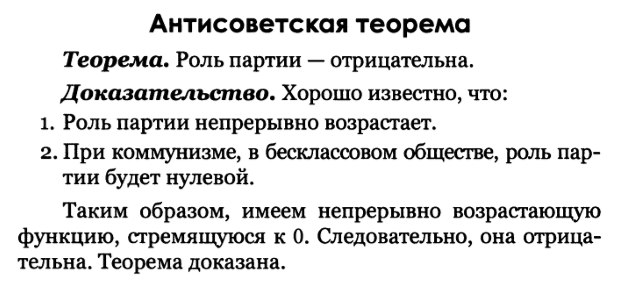
\includegraphics[width=\textwidth]{part}
    \caption{Актуально во все времена}
\end{figure}
\begin{itemize}
    \item ... написании брошюры: "Размышление о бренности бытия в поезде/автомобиле/самолёте. Самоучитель для домохозяек."
    \item ... создании фирмы: "Профилактические люли: Быстро! Эффективно! Недорого!"
    \item ...  создании методики по определению реального уровня образования конкретного человека (польза для начальников при подборе персонала). Основание -- анализ ответов на простые детские вопросы.
    Например:
        \begin{itemize}
            \item что такое число?
            \item почему небо синее, а облака белые?
            \item куда девается грипп летом?
            \item откуда так много пород собак?
            \item почему пицца круглого, а коробка квадратного сечения?
            \item какова молния на вкус?
            \item почему люди такие идиоты?
        \end{itemize}
    \item ... об антиметоде направленный на определения умственных способностей начальников.    
    \item ... создании неогоголианского стиля написания книг:\\
        \emph{Короче, залез я в холодильник, взял помидору, огурец, зелень, хотел салат сделать. Ну естественно, 
            салат надо делать с майонезом, иначе какой нормальный человек его есть будет. Я все нарезал и вдруг 
            понял, что майонез я забыл, чёртов слоупок. Открываю холодильник, беру майонез и вдруг понимаю, что 
            передо мной лежит сало. Никогда раньше не ел сала, а тут вдруг захотелось, ну думаю, раз захотелось, 
            почему бы и не съесть. Пока заправил салат, нарезал сало, все как положено, покушал и тут вдруг все 
            перефарбувалося у жовтоблакитний колiр, гул та рокiт, їбать у сраку, що за гомно, нічого не 
            зрозуміло, вилазить із земли Тарас Шевченко и каже якусь хуйню про москалів і мораль старий педаль, 
            хулі йому у землі не лєжалось блядь? Відтепер окрім української мови я ніхуя не розумію. Здається 
            сало було прокляте.}
    \item ... выявлении корреляции между творческим подъёмом и уровнем неблагоприятности внешних условий.
    \item ... создании аналога тепловизора, работающего на основе соприкосновения различных участков тела с воздушными массами проградуированной температуры.
    \item ...создании специальностей: критик и доработчик идей для стартапов.
    \item ...создании самой честной партии: партии жуликов и воров.
    \item ...нового боевого искусства: вУфу.
\end{itemize}
% - надо размер рекламы подобрать
% - это надо будет обсудить
\begin{figure}[ht!]
    \centering
    
\includegraphics[width=0.6\textwidth]{hellisemptyAllthedevilsarehere}
    \caption{Мы ждём вас!}
\end{figure}

%тут надо продумать какое-нибудь спец. оформление
Любезно предоставляем гипотетическим читателям возможность подумать над следующей гипотетической теорией:
N-мерных (для начала гильбертовых) пространств, где N<0.\\
Ваши идеи (и наработки) отправляйте \href{http://www.abelprize.no/}{сюда} для вознаграждения.

\subsection{Бредовые аналоги аналогов}
\begin{itemize}
\item порошковое `кофе`, `молоко` \( \to \) чай - щи - яичница - ...
\item катер на `воздушной` подушке \( \to \) водной - земляной - облачной - ...
\item `жидкое` электричество \( \to \) газообразное - твёрдое - мягкое - ...
\item `водоотталкивающая` ткань \( \to \) водопритягивающая (для садов и огородов)
\item `взбитые` сливки \( \to \) молотые - плавленные - жаренные - варёные - ...
\item `радио-`, `теле-` антенна \( \to \) торсионная - эфирная - вакуумная - ... (+ аналогично со спутником)
\end{itemize}
\subsection{Бредовые гибриды}

\begin{figure}[ht!]
    \centering
    
\includegraphics[width=0.6\textwidth]{hubr}
    \caption{гибрид --- кошка и геккон}
\end{figure}

\begin{itemize}
\item кошка + мышь, заяц + волк
\item человек + скунс, человек + ленивец, человек + жираф, ...
\item гепард + крокодил, гепард + жираф, гепард + ленивец, ...
\item скунс + анти скунс (если такой был бы)
\item помидор + огурец + лук + ... = готовый салат
\item змея с ушами

\end{itemize}
